\documentclass[letterpaper,landscape]{slides}
%\documentclass[letterpaper,portrait]{slides}
\usepackage{boxedminipage}

%\input /u/rhl/TeX/pdf.tex
\input pdf.tex

\newif\ifTalk\Talktrue		% We generating a talk, not printing
%\Talkfalse			% no; we're really printing

%\pagestyle{empty}
\setlength{\topmargin}{-1in}
\setlength{\textheight}{7.5in}
\setlength{\textwidth}{9in}
\setlength{\oddsidemargin}{0pt}
\setlength{\oddsidemargin}{0pt}

%\onlyslides{1-3,4,10-9999}
%\onlyslides{26-9999}

\begin{document}

\newcommand{\XXX}[1]{\textbf{XXX} #1}
\newcommand{\colour}[1]{\color{#1}}


\def\eq#1{\begin{equation} \color{blue} #1 \end{equation}}
\def\vx{{\bf x}}
\def\vv{{\bf v}}
\def\b#1{{\bf  #1}}
\def\p{\partial}
\def\th{^{th}}
\def\msun{{\rm\,M_\odot}}
\def\bnabla{{\bf\nabla}}
\def\dint{\int\!\!\!\int}
\def\d{{\rm d}}
\def\i{{\rm i}}
\def\ddt#1{{\rm{d} #1\over {\rm dt}}}
\def\ddtS#1{{\rm{d^2} #1\over {\rm dt^2}}}
%\lta and \gta produce > and < signs with twiddle underneath
\def\spose#1{\hbox to 0pt{#1\hss}}
\def\lta{\mathrel{\spose{\lower 3pt\hbox{$\mathchar"218$}}
     \raise 2.0pt\hbox{$\mathchar"13C$}}}
\def\gta{\mathrel{\spose{\lower 3pt\hbox{$\mathchar"218$}}
     \raise 2.0pt\hbox{$\mathchar"13E$}}}
\def\mspace{\hbox{\quad}}

\def\deffn#1{{\bf#1}}\def\eqs#1{equations \rf#1}


\newcount\itemCnt\itemCnt=0
\newcommand{\nitem}{%
  \global\advance\itemCnt by 1
  ~\vskip0cm\the\itemCnt.\qquad}

\definecolor{orange}{rgb}{1.0, 0.5, 0.0}
\definecolor{purple}{cmyk}{0.4, 0.8, 0.3, 0.0}


%%%%%%%%%%%%%%%%%%%%%%%%%%%%%%%%%%%
\newcommand{\onepic}[6]{%
\begin{slide}
     \begin{center}
        \begin{minipage}{#1in}
            {\large \color{blue} #6}
            \phantom{x} \vskip #2in
            \phantom{x} \hskip #3in
            {\scalebox{#4}{\includegraphics{#5}}}   
        \end{minipage}
     \end{center}
    \vfill
\end{slide}
}


%%%%%%%%%%%%%%%%%%%%%%%%%%%%%%%%%%%
\newcommand{\picslide}[7]{%
  \begin{slide}
     \begin{center}
        \begin{minipage}{#5in}
            \hskip #6in
            \hskip -1in
            {\scalebox{#4}{\includegraphics{#1.#2}}}
            \vskip #7in~
            {\large \color{blue} #3}
        \end{minipage}
     \end{center}
     \vfill
  \end{slide}
}
%%%%%%%%%%%%%%%%%%%%%%%%%%%%%%%%%%%
 

%%%%%%%%%%%%%%%%%%%%%%%%%%%%%%%%%%%
\newcommand{\Spicslide}[7]{%
  \begin{slide}
     \begin{center}
        \begin{minipage}{#5in}
            \vskip #6in
            \hskip #7in
            {\scalebox{#4}{\includegraphics{#1.#2}}}
        \end{minipage}
     \end{center}
     \vfill
  \end{slide}
}
%%%%%%%%%%%%%%%%%%%%%%%%%%%%%%%%%%%
 


%------------------------------------------------------------------------------
%------------------------------------------------------------------------------

\begin{slide}

\phantom{x}
\vskip -2in
\begin{center}
\bfseries
{\large {\color{blue} Astr 511: Galaxies as galaxies}}
\end{center}

{\centerline {{\color{blue} 
Winter Quarter 2017, University of Washington}}}
{\centerline {{\color{blue} 
Mario Juri\'{c} \& \v{Z}eljko Ivezi\'{c} }}}

\vskip 1.6in

{\centerline {\huge {\color{red}      Lecture 14:             }}}
\vskip 0.2in 
{\centerline {\Large {\color{blue} Open questions in galactic astronomy }}}
{\centerline {\Large {\color{blue} and modern sky surveys }}}

\vfill
\end{slide}
%------------------------------------------------------------------------------



%------------------------------------------------------------------------------
% TWO-SIDED PAGE 
\begin{slide}

\hbox to \hsize{
\begin{minipage}[t]{16cm}
\begin{center}
\vskip -1.7in
\scalebox{0.4}{\hskip -3.3in \includegraphics{figures/MW_Poster18x24_noText.pdf}}

\end{center}

\end{minipage}

\begin{minipage}[t]{8cm}
\begin{center}
%{\large \color{red} The three basic stellar distribution functions:}
\end{center}
\vskip 0.3in
\begin{enumerate}
\item {\bf Number density}
\item  {\bf Metallicity}
\item  {\bf Kinematics} 
\end{enumerate}     

{\large These three distribution functions provide
observational constraints for the model selection (models for
galaxy formation and evolution)}

{\large \color{blue} How well do we know these distribution functions?} 




\end{minipage}}
\vfill 
\end{slide}
%------------------------------------------------------------------------------


%------------------------------------------------------------------------------
\begin{slide}
\begin{center}
\bfseries
{\large {\color{blue} Two major goals for the Milky Way models} }
\end{center}
\begin{enumerate}
            \item {\bf The origin and evolution of thin and thick disks:} can we generate a model
                  that simultaneously reproduces the spatial, kinematic and chemical distributions? 
             \item {\bf The halo structure:} can we generate a model that simultaneously  
                             reproduces spatial and kinematic structure and substructure
                              (including streams and dark matter)? 
\end{enumerate}
\vskip -0.47in
{\color{red} \bf Examples of related observational questions:}
\vskip -0.7in
  \begin{itemize}
  \item {\color{blue} How do the properties of the bulge compare to those of the disk and the halo?} 
   \item {\color{blue} What are the shapes of the density and velocity dispersion profiles of the stellar halo, and 
                do they remain constant with increasing distance (and/or declining metallicity)?}
  \item {\color{blue} What fraction of halo is in substructures? }
\end{itemize}


\vfill
\end{slide}
 
%------------------------------------------------------------------------------




%------------------------------------------------------------------------------
% TWO-SIDED PAGE 
\begin{slide}

\hbox to \hsize{
\begin{minipage}[t]{12cm}
\vskip -1in
\begin{center}
{\large \color{red}  $[\alpha/Fe]$ vs. $[Fe/H]$ distribution for disk stars
from SDSS APOGEE survey}
\begin{itemize}
\item Anders et al. (2014, A\&A 564, A115): strong variation of
the $[\alpha/Fe]$ vs. $[Fe/H]$ distribution with the distance from the
Galactic center
\end{itemize} 
\vskip 0.7in 
\scalebox{0.9}{\hskip -0.7in \includegraphics{figures/Anders2014.png}}
\end{center}
\end{minipage}


\begin{minipage}[t]{12cm} 
\begin{itemize}
\item Solar radius (8 kpc) is a transition zone between the ``inner''
and ``outer'' disks
\item The inner disk is dominated by the thick disk and the metal-rich part
of the thin disk
\item The outer disk is dominated by the metal-poor part
of the thin disk
\end{itemize} 
\end{minipage}}
\vfill 
\end{slide}
%-----------------------------------------------------------------------------



%------------------------------------------------------------------------------
% TWO-SIDED PAGE 
\begin{slide}

\hbox to \hsize{
\begin{minipage}[t]{12cm}
\vskip -1in
\begin{center}
{\large \color{red}  $[\alpha/Fe]$ vs. $[Fe/H]$ distribution for disk stars
from SDSS APOGEE survey}
\vskip 0.4in 
\scalebox{0.76}{\hskip -1.4in \includegraphics{figures/Hayden2015.png}}
\end{center}
\end{minipage}

\begin{minipage}[t]{12cm} 
\begin{itemize}
\item Hayden et al. (2015, ApJ 808, 132): strong variation of
the $[\alpha/Fe]$ vs. $[Fe/H]$ distribution with both $R$ and $Z$! 
\end{itemize} 
\end{minipage}}
\vfill 
\end{slide}
%-----------------------------------------------------------------------------



%------------------------------------------------------------------------------
% TWO-SIDED PAGE 
\begin{slide}

\hbox to \hsize{
\begin{minipage}[t]{10cm}
\begin{center}
\vskip -0.75in
\scalebox{0.05}{\hskip -10.4in 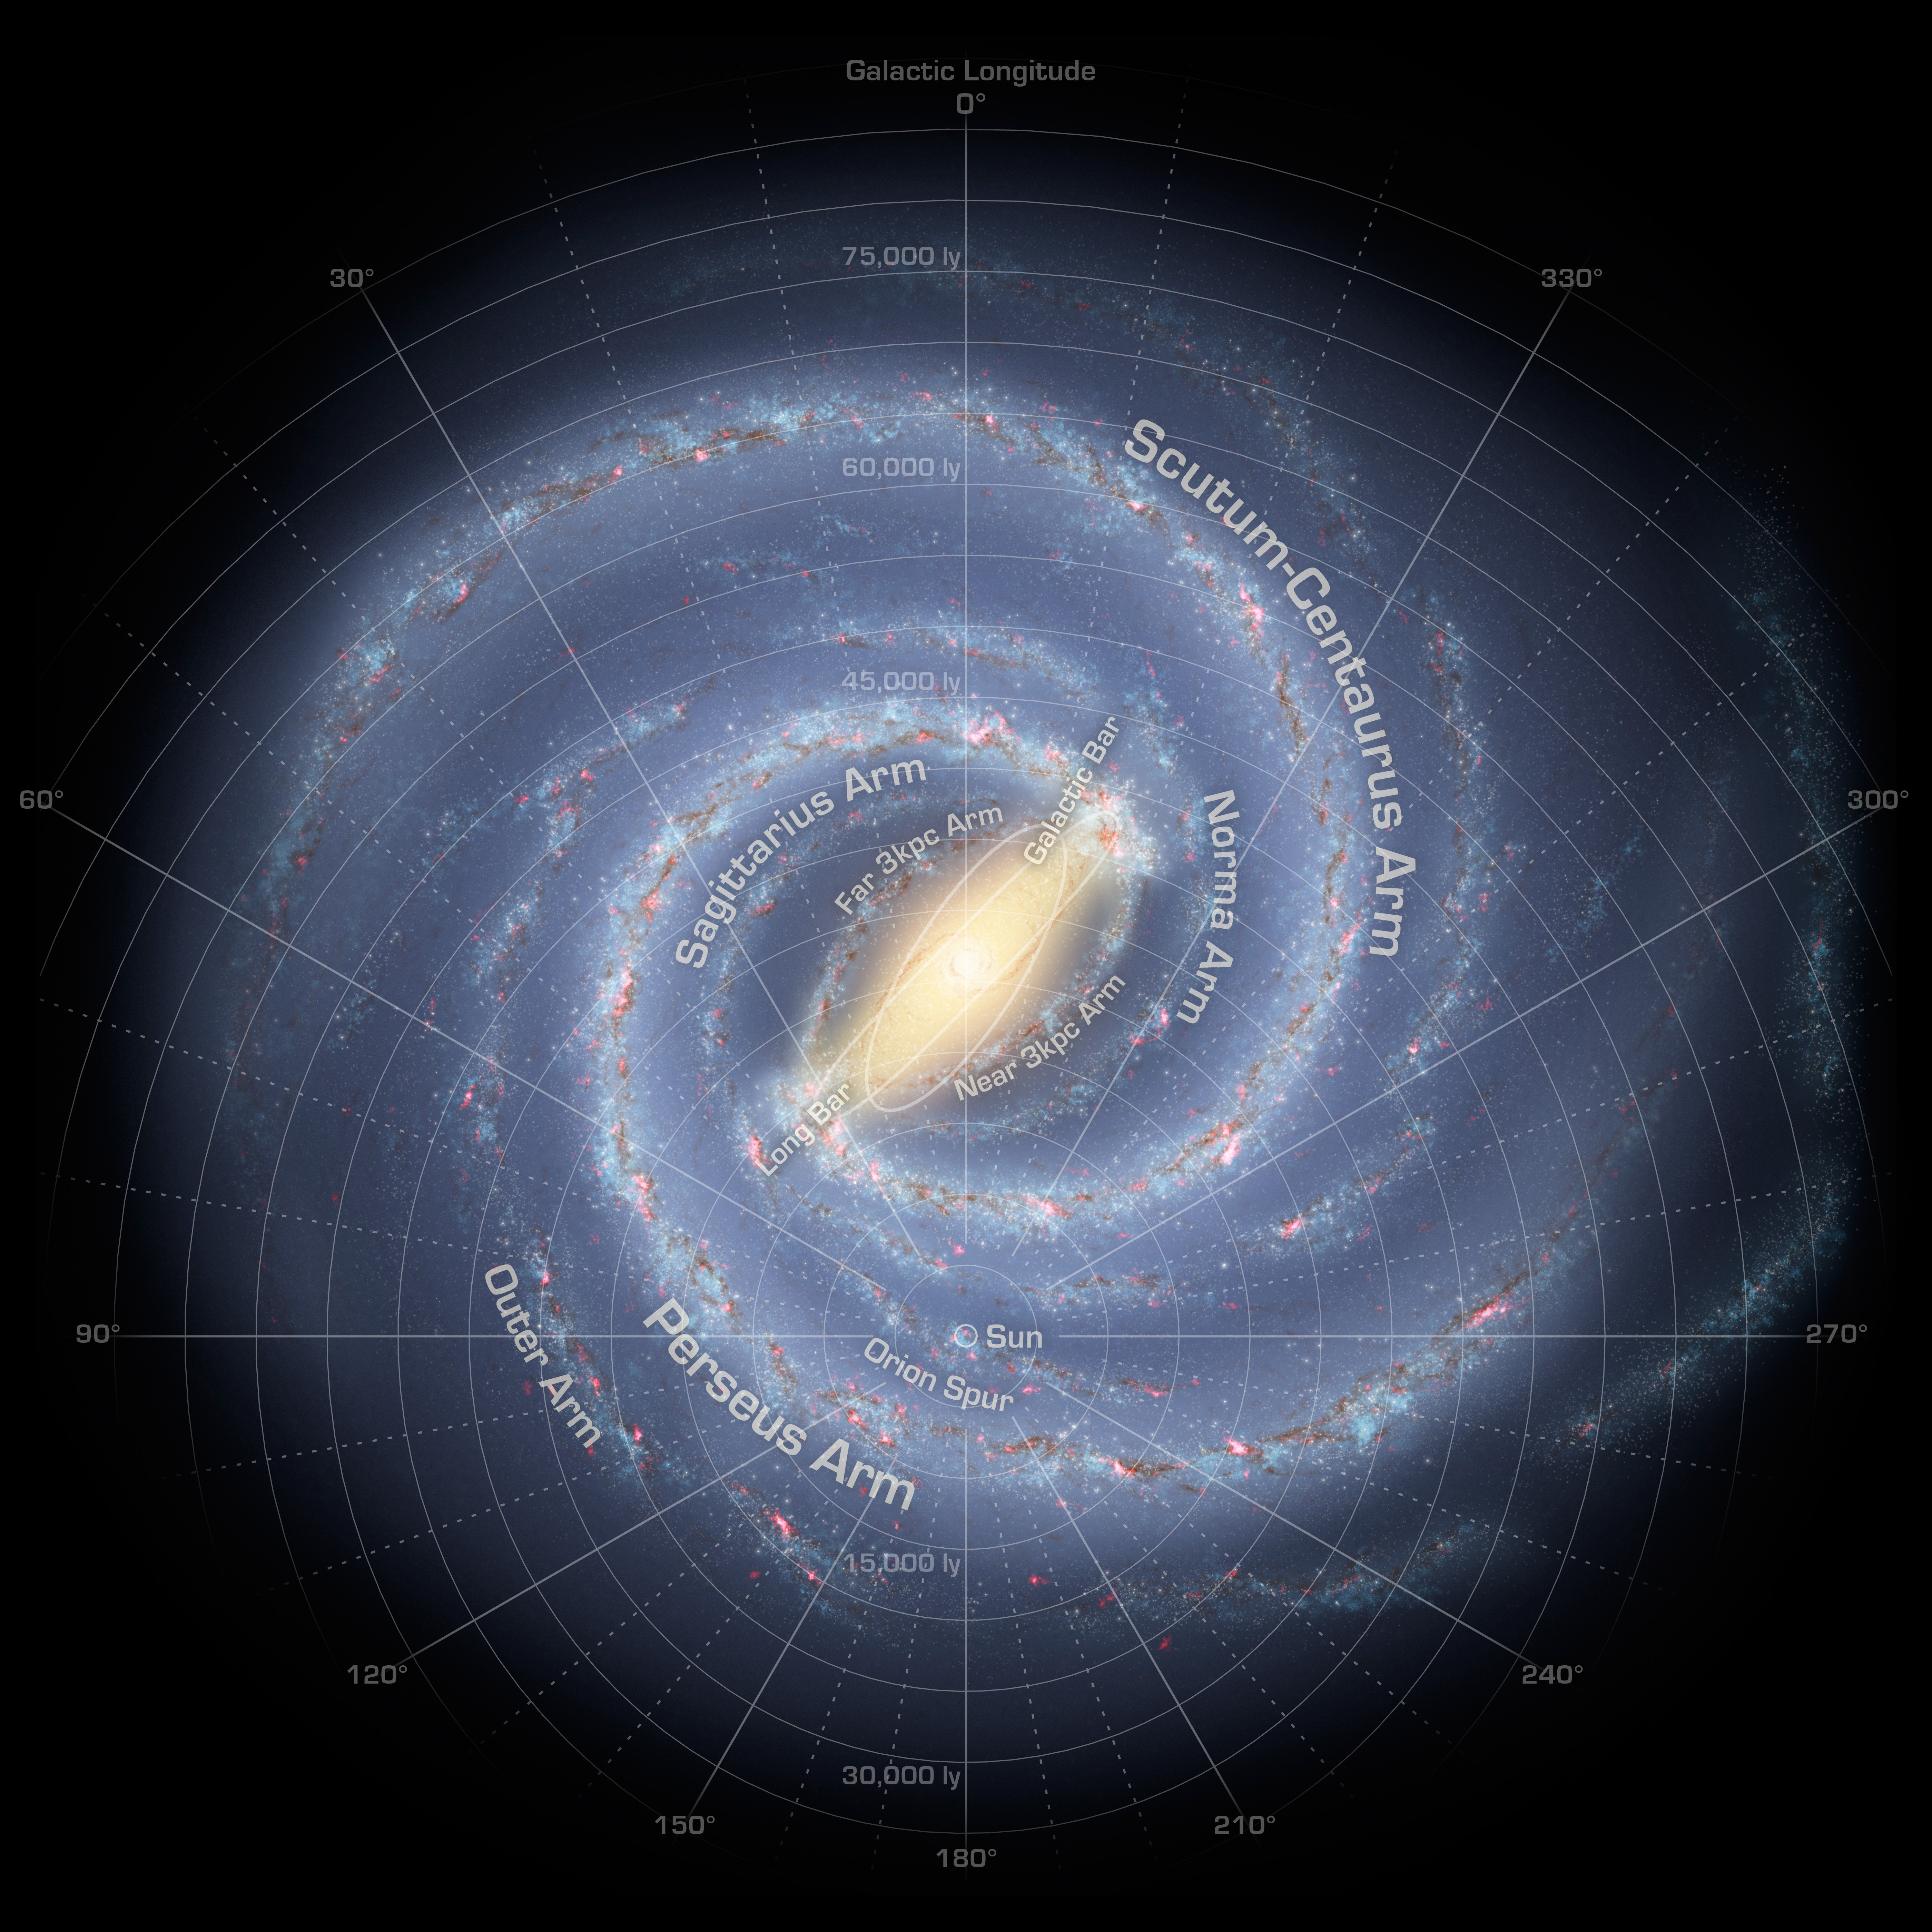
\includegraphics{figures/MWplaneAnnotated.jpg}}
\vskip 0.1in
\scalebox{0.37}{\hskip -2.8in \includegraphics{figures/snapshot1.jpg}}
\end{center}
\end{minipage}

\begin{minipage}[t]{14cm}
\begin{center}
\vskip -1in
{\large \color{red} Outer halo studies: RR Lyrae from SDSS Stripe 82}
\end{center}

\begin{itemize}
\item {\bf Top left:} the disk structure (artist's conception based on the Spitzer and
      other surveys of the Galactic plane)
\item {\bf Bottom left:} the halo density (multiplied by $R^3$; yellow and red are overdensities
      relative to mean $\rho(R)\propto R^{-3}$ density) as traced by
      $\sim$500 RR Lyrae from SDSS Stripe 82
      (Watkins et al; Sesar et al. 2009), compared in scale to the top panel
\item {\color{blue} Conclusions:} the spatial distribution of halo stars is highly
inhomogeneous (clumpy); when averaged, the stellar volume density decreases
as $\rho(R)\propto R^{-3}$.
\end{itemize}     

\end{minipage}}
\vfill 
\end{slide}
%------------------------------------------------------------------------------



%------------------------------------------------------------------------------
% TWO-SIDED PAGE 
\begin{slide}

\hbox to \hsize{
\begin{minipage}[t]{11cm}
\begin{center}
\vskip -5.8in
\scalebox{0.82}{\hskip -1.4in \includegraphics{figures/f13.pdf}}
\vskip 0.2in
\scalebox{0.82}{\hskip -1.3in \includegraphics{figures/large-fg22.jpg}}
\end{center}
\end{minipage}

\begin{minipage}[t]{13cm}
\begin{center}
\vskip -1in
{\large \color{red} Outer halo studies: RR Lyrae from SDSS Stripe 82}
\end{center}

\begin{itemize}
\item {\bf Top left panels:} four regions selected by R.A.; points: observed 
     density, blue line: fit from Sesar et al. (2009); red lines: fit from 
       Watkins et al. (2009); similar results for 2016 candidate
           RR Lyrae from SEKBO survey (Keller et al. 2008); 
\item {\bf Bottom left panel:} Oosterhof I and II profiles for 838 LONEOS
           RR Lyrae from Miceli et al (2008); confirmed by stripe 82 RR Lyrae 
\item {\color{blue} {\bf Conclusions:} The density profile steepens beyond $\sim$30
     kpc; within 30 kpc, the profile for Oosterhof II subset is steeper}
\end{itemize}     

\end{minipage}}
\vfill 
\end{slide}
%------------------------------------------------------------------------------




%------------------------------------------------------------------------------
% TWO-SIDED PAGE 
\begin{slide}

\hbox to \hsize{
\begin{minipage}[t]{10cm}
\begin{center}
\vskip -3.75in
\scalebox{0.9}{\hskip -1.4in \includegraphics{figures/f23.pdf}}
\end{center}
\end{minipage}

\begin{minipage}[t]{14cm}
\begin{center}
\vskip -1in
{\large \color{red} Outer halo studies: main-sequence stars}
\end{center}

\begin{itemize}
\item Sesar et al. (2009): co-added SDSS Stripe 82 data enable 
  mapping with numerous main-sequence stars out to $\sim$30 kpc
\item {\bf Top left:} Observed density map
\item {\bf Top right:} Galfast model prediction
\item {\bf Bottom left:} Data/model ratio, overdensity is the Sgr tidal stream
\item {\bf Bottom right:} Data/model ratio along the celestial equator
\item {\color{blue} Evidence for steepening of the density profile beyond 
    $\sim$20 kpc from the Galactic center}
\item Consistent conclusion with the RR Lyrae spatial profile
\end{itemize}     

\end{minipage}}
\vfill 
\end{slide}
%------------------------------------------------------------------------------




%------------------------------------------------------------------------------
% TWO-SIDED PAGE 
\begin{slide}

\hbox to \hsize{
\begin{minipage}[t]{10cm}
\begin{center}
\vskip 2.5in
\scalebox{0.75}{\hskip -2.4in \includegraphics{figures/20071212dblhalo.jpg}}
\vskip -13.5in
\scalebox{0.8}{\hskip -1.7in \includegraphics{figures/f24.pdf}}
\end{center}
\end{minipage}

\begin{minipage}[t]{14cm}
\begin{center}
\vskip -1in
{\large \color{red} Outer halo studies: main-sequence stars}
\end{center}

\begin{itemize}
\item Evidence for steepening of the density profile beyond 
    $\sim$20 kpc from the Galactic center
\item {\color{blue} Top left: evidence for drop in metallicity of smooth background
       halo beyond $\sim$20-30 kpc}
\item {\color{red} However, high surface-brightness overdensities have 
     higher $[Fe/H]$, top right} Supports simulation-based results by, e.g., 
     Johnston et al. (2008) and Zolotov et al. (2009)
\item Agrees with indirect results based on kinematics from Carollo 
     et al. (2007) and Carollo et al. (2010), bottom panel
\end{itemize}     

\end{minipage}}
\vfill 
\end{slide}
%------------------------------------------------------------------------------











%------------------------------------------------------------------------------
\begin{slide}
\begin{center}
{\large \color{red} 
                     (Dark) Halo mass density profile  }
\end{center}

The Jeans equation for a steady-state rotationally invariant spherical system (see Lecture 7):

\begin{eqnarray}
\color{blue} {1 \over \nu}  {d(\nu \sigma_r^2) \over dr } + {2 \beta \sigma_r^2 \over r}  & = &
 \color{blue} -{d \Phi \over dr}  \nonumber
\end{eqnarray}
where $\beta = 1-(\sigma_\theta/\sigma_r)^2$ (note that here ``r'' is the spherical galactocentric radius). 

With $d\Phi/dr=GM(r)/r^2$, we can translate SDSS results to a constraint on $M(r)$. For example,
\begin{itemize}
\item Juri\'{c} et al. (2008) obtained for halo: $\nu(r) \propto r^{-2.8}$
\item Bond et al. (2010) list $\sigma_r=141$ km/s,  $\sigma_\theta=75$ km/s,  and $\sigma_\phi=85$ km/s
\end{itemize}

\vfill
\end{slide}





%------------------------------------------------------------------------------
\begin{slide}
\begin{center}
{\large \color{red} 
                     (Dark) Halo mass density profile: spherical case  }
\end{center}

 Ignoring for a moment that Juri\'{c} et al. (2008) obtained an oblate halo ($c/a=0.64$), and that
$\sigma_\theta$ and $\sigma_\phi$ are not equal (assume $\beta=0.68$),  it is easy to show that 
{\color{blue} $M(r) \propto r$.}

This $M(r)$ behavior implies a logarithmic gravitation potential $\Phi(r) = v_c^2 \, ln(r/r_c)$, where
$v_c$ is the circular velocity, and $r_c$ is a characteristic spatial scale. 

More importantly,
we also get $\rho(r) \propto r^{-2}$, where $\rho(r)$ includes {\bf all} the matter! 

This profile is the so-called ``iso-thermal'' profile and implies a flat rotation curve. 

{\color{blue} But what about the fact that we ignored departures from spherical 
symmetry for the halo density law?}  See Loebman et al. (2012, ApJ 758, L23)
and Lecture 10. 


\vfill
\end{slide}



%------------------------------------------------------------------------------



%------------------------------------------------------------------------------
% TWO-SIDED PAGE 
\begin{slide}

\hbox to \hsize{
\begin{minipage}[t]{12cm}
\begin{center}
\vskip -0.2in
\scalebox{0.8}{\hskip -1.4in \includegraphics{figures/gnedin1.jpg}}
Gnedin et al.  (2010, ApJ 720, L108) 
\end{center}
\end{minipage}

\begin{minipage}[t]{12cm}
\begin{center}
\vskip -0.9in
     {\large \color{red} Halo radial velocity dispersion: profile at large radii  }
\end{center}

\begin{itemize}
\item {\color{blue} Does the radial velocity dispersion vary in the outer halo?} 
\item  Data show only a little bit of gradient between $\sim10$ kpc and $\sim$100 kpc: 
Gnedin et al. (2010) get a power-law index of $-0.08$. 
\item If recent SDSS-based values from Bond et al. (2010) and Smith et al. (2009) are added, then the
power-law index becomes $-0.12$.
\item {\bf We need better kinematic data in the 10-100 kpc distance range.}
\end{itemize}     

\end{minipage}}

\vfill 
\end{slide}
%------------------------------------------------------------------------------



%------------------------------------------------------------------------------

\begin{slide}

\begin{center}
\bfseries
\large \colour{red} Tentative Summary of Direct Halo Measurements
\end{center}
\vskip 0.2in
\begin{enumerate}
 \item {\color{blue} \bf $\rho(R,Z,\phi)$:} 
   \begin{itemize}
     \item Within $\sim$10 kpc traced by main-sequence stars;
         oblate ($q=0.64\pm0.1$), $\rho \sim 1/R^3$ ($n=2.8\pm0.2$)
     \item Within $\sim$100 kpc traced by RR Lyrae stars; 
         a steeper slope beyond 30 kpc and much more substructure,
         extends to at least $\sim$100 kpc, within 30 kpc Oosterhof II
         subset have a steeper slope 
   \end{itemize}    
 \item {\color{blue} \bf $[Fe/H]$:}
   \begin{itemize}
     \item Within $\sim$10 kpc traced by 
         main-sequence stars; uniform gaussian distribution (gradient 
         $<0.01$ dex/kpc) centered on $[Fe/H]=-1.5$ with a dispersion 
         of 0.3 dex
     \item Beyond $\sim$20-30 kpc, $[Fe/H]$ for the background
         diffuse population probably decreases; however, for high 
         surface brightness substructure $[Fe/H]> -1.5$ (Sgr trailing 
         tidal tail: $[Fe/H]= -1.2$, Monoceros stream: $[Fe/H]= -1.0$)
   \end{itemize}    
 \item {\color{blue} \bf Kinematics:} 
   \begin{itemize}
     \item Within $\sim$10 kpc traced by main-sequence stars, no
	   rotation to within 10-20 km/s, velocity ellipsoid
           aligned with the spherical coordinate system: 
           $\sigma_R=140$ km/s, $\sigma_\phi=85$ km/s,
	   $\sigma_\theta=75$ km/s
     \item Limited data beyond 10 kpc; based on a heterogeneous
        sample of $\sim$250 objects, it appears that beyond $\sim$30 kpc 
        the radial velocity dispersion is decreasing with $R$
        (to $\sim50$ km/s at $\sim$120 kpc).      
   \end{itemize}    
\end{enumerate}    

{\color{red} ``We need mo' data!'' }

\vfill 
\end{slide}


%------------------------------------------------------------------------------



\end{document}



